\begin{song}{title=\predtitle\centering Dokud se zpívá \\\large Jaromír Nohavica  \vspace*{-0.3cm}}  %% sem se napíše jméno songu a autor
\begin{centerjustified}
\nejnejvetsi

\sloka
	^{C}Z Těšína ^{Emi\,\,\,\,\,}vyjíždí ^{Dmi7\z}vlaky~co ^{F{\color{white}aaaaaa}C}čtvrthodinu, ^{Emi\,Dmi7\,G}

	včera jsem nespal a ani dnes nespočinu,

	^{F}svatý ^{G}Medard, můj ^{C}patron, ^{\z Ami\:\:\:}ťuká~si~na ^{{\color{white}aa}G}čelo,

	ale ^{F}dokud se ^{G}zpívá, ^{F}ještě se ^{G{\color{white}aaaa}C}neumřelo. ^{Emi\,Dmi7\,G}

\sloka
	Ve stánku koupím si housku a slané tyčky,

	srdce mám pro lásku a hlavu pro písničky,

	ze školy dobře vím, co by se dělat mělo,

	ale dokud se zpívá, ještě se neumřelo.

\sloka
	Do alba jízdenek lepím si další jednu,

	vyjel jsem před chvílí, konec je v nedohlednu,

	za oknem míhá se život jak leporelo,

	ale dokud se zpívá, ještě se neumřelo.

\sloka
	Stokrát jsem prohloupil a stokrát platil draze,

	houpe to, houpe to na housenkové dráze,

	i kdyby supi se slítali na mé tělo,

	tak dokud se zpívá, ještě se neumřelo.

\sloka
	Z Těšína vyjíždí vlaky až na kraj světa,

	zvedl jsem telefon a ptám se: \uv{Lidi, jste tam?}

	A z veliké dálky do uší mi zaznělo,

	/: že dokud se zpívá, ještě se neumřelo. :/


\end{centerjustified}

\centering
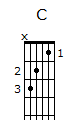
\includegraphics[width=3cm]{../Akordy/c}
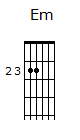
\includegraphics[width=3cm]{../Akordy/em}
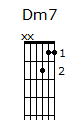
\includegraphics[width=3cm]{../Akordy/dm7}
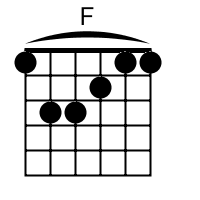
\includegraphics[width=3cm]{../Akordy/f}
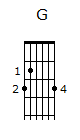
\includegraphics[width=3cm]{../Akordy/g}

\setcounter{Slokočet}{0}
\end{song}
